\chapter{Born 级数与 Lippmann--Schwinger 方程 (Born Series)}\label{ch:born}

前一章我们引入了 Green 算符 $G_0(z)=(z-\Hmat_0)^{-1}$ 与全空间 Green 算符 $G(z)=(z-\Hmat)^{-1}$，并得到 Lippmann--Schwinger 方程
\begin{equation}
\Tmat(z)=\Vmat+\Vmat\,G_0(z)\,\Tmat(z),\qquad
G(z)=G_0(z)+G_0(z)\,\Vmat\,G(z).
\label{eq:LS-recall}
\end{equation}
在能壳上 (on-shell) 取 $z=E_p+\rmi 0$, 即可得到 $T$ 矩阵元
\begin{equation}
t(\bm p'\!\leftarrow\bm p)=\matel{\bm p'}{\Tmat(E_p+\rmi 0)}{\bm p},
\end{equation}
它直接给出散射振幅 $f(\bm p'\!\leftarrow\bm p)=-(2\pi)^2 m\,t(\bm p'\!\leftarrow\bm p)$ 与微分截面。本章的目标是构造 \eqref{eq:LS-recall} 的迭代解 (Born 级数), 讨论其收敛性、最低阶 (玻恩) 近似的物理图像与适用范围, 并通过 Yukawa 势、电子-原子散射等例子加以说明。最后我们指出 Born 级数也可以视为相互作用图像下 $S$ 算符的微扰展开, 给出对应的 Feynman 图规则。

\section{Born 级数的形式构造}\label{sec:born-formal}

\subsection{从 Lippmann--Schwinger 方程出发的迭代}

为了引入合适的小参数, 把相互作用部分写成 $\Vmat\to\lambda\Vmat$, 把 $\lambda$ 看作从 $V$ 中抽出的耦合常数, 最后取 $\lambda\to 1$. 哈密顿量为
\begin{equation}
\Hmat=\Hmat_0+\lambda\Vmat.
\end{equation}
对应的 Lippmann--Schwinger 方程
\begin{equation}
\Tmat(z)=\lambda\Vmat+\lambda\Vmat\,G_0(z)\,\Tmat(z)
\label{eq:LS-lambda}
\end{equation}
是 $\Tmat$ 的算符方程。形式上把它解出来得
\begin{equation}
\bigl[1-\lambda\Vmat\,G_0(z)\bigr]\Tmat(z)=\lambda\Vmat
\;\Longrightarrow\;
\Tmat(z)=\bigl[1-\lambda\Vmat\,G_0(z)\bigr]^{-1}\lambda\Vmat
=\sum_{n=0}^{\infty}\bigl(\lambda\Vmat\,G_0(z)\bigr)^{n}\lambda\Vmat.
\label{eq:born-T}
\end{equation}
若把 $\Tmat(z)$ 关于 $\lambda$ 做形式幂级数展开
\begin{equation}
\Tmat(z)=\sum_{n=0}^{\infty}\lambda^{n}\Tmat^{(n)}(z),
\end{equation}
比较 \eqref{eq:LS-lambda} 两边各阶的系数可得
\begin{equation}
\Tmat^{(0)}=0,\quad \Tmat^{(1)}=\Vmat,\quad
\Tmat^{(n)}=\Vmat\bigl(G_0\Vmat\bigr)^{n-1}=\bigl(\Vmat G_0\bigr)^{n-1}\Vmat,\;n\ge 1.
\end{equation}
取 $\lambda\to 1$ 给出 \emph{Born 级数}
\begin{equation}
\boxed{\;\Tmat(z)=\Vmat+\Vmat G_0(z)\Vmat+\Vmat G_0(z)\Vmat G_0(z)\Vmat+\cdots
=\sum_{n=0}^{\infty}\Vmat\bigl(G_0(z)\Vmat\bigr)^{n}\;}
\label{eq:born-series}
\end{equation}
对应于波函数与 Green 算符的级数为
\begin{align}
\ket{\psi^{\pm}}&=\ket{\phi}+G_0^{\pm}\Vmat\ket{\phi}+G_0^{\pm}\Vmat G_0^{\pm}\Vmat\ket{\phi}+\cdots,\\
G(z)&=G_0(z)+G_0(z)\Vmat G_0(z)+G_0(z)\Vmat G_0(z)\Vmat G_0(z)+\cdots .
\end{align}

\subsection{On-shell $T$ 矩阵元的展开}

把 \eqref{eq:born-T} 投影到自由动量本征态 $\ket{\bm p}$, 并取 $z=E_p+\rmi 0$:
\begin{equation}
t(\bm p'\!\leftarrow\bm p)
=\lambda\matel{\bm p'}{V}{\bm p}
+\lambda^{2}\matel{\bm p'}{V\,G_0(E_p+\rmi 0)\,V}{\bm p}+\cdots .
\label{eq:T-expansion}
\end{equation}
令 $\lambda\to 1$, 第 $n$ 项即 $t^{(n)}(\bm p'\!\leftarrow\bm p)$.

\begin{remark}[Born 级数的一般性质]
\begin{itemize}
  \item Born 级数不一定收敛。
  \item 即使收敛, 也不一定收敛得很快, 前几阶不一定给出主要贡献。
  \item 在某些情形下收敛得足够快, 特别是高能或者势足够弱时, 最低阶的几项可能就给出主要贡献。
  \item 即便仅知道收敛性, Born 级数也可以用来在理论上推出散射振幅的一些一般性质 (例如解析性、幺正性等)。
  \item 当确实没有别的方法时, Born 近似往往是唯一可用的工具。
\end{itemize}
\end{remark}

\section{收敛性条件}\label{sec:convergence}

我们期望当算符 $\lambda\Vmat\,G_0$ 在某种范数下足够 “小” 时, \eqref{eq:born-T} 中的几何级数收敛。直观上, 有两种使其变小的途径:
\begin{enumerate}
  \item $\lambda$ 充分小, 即耦合常数足够弱;
  \item 能量 $E_p$ 充分大, 此时 $G_0=(z-\Hmat_0)^{-1}$ 在算符范数意义下变小。
\end{enumerate}
在适当条件下 (例如 $V$ 满足前章中保证 $T$ 矩阵存在的条件), 可以严格证明下列两条结论。

\begin{theorem}[弱耦合下的收敛性]\label{thm:weak-coupling}
对于任何势 $V$, 存在 $\bar\lambda>0$ 使得对所有 $|\lambda|<\bar\lambda$ 与所有 $\bm p,\bm p'$, Born 级数 \eqref{eq:T-expansion} 收敛到正确的 on-shell $T$ 矩阵元. $\lambda$ 越小, 收敛越快, 第一项 (Born 近似) 给出主要贡献。
\end{theorem}

\begin{theorem}[高能区的收敛性]\label{thm:high-energy}
对任何势 $V$, 存在 $\bar E$ 使得当 $E>\bar E$ 时, Born 级数在 $\lambda=1$ 时都收敛. $E$ 越大, 收敛越快; 对足够大的 $E$, 第一项 Born 近似给出主要贡献。
\end{theorem}

\begin{remark}[束缚态与收敛性的关系]
若 $\lambda$ 足够小使得 Born 级数对所有 $E>0$ 都收敛, 那么 $\lambda V$ 没有束缚态 (Green 算符 $G(z)$ 在 $z=E_p+\rmi 0$ 附近正则). 反过来, 如果势 $V$ 支持束缚态, 那么相应的 Born 级数无法对所有正能量都收敛 —— 因为某些 $E>0$ 邻域内 $G$ 的解析延拓附近会出现极点或不规则性的痕迹, 而 \eqref{eq:born-T} 中的几何级数无法描述这种结构。
\end{remark}

\section{第一阶 Born 近似}\label{sec:first-born}

\subsection{$T$ 矩阵元与散射振幅}

仅保留 \eqref{eq:T-expansion} 的第一项就得到 \emph{Born 近似 (first Born approximation)}:
\begin{equation}
t^{(1)}(\bm p'\!\leftarrow\bm p)=\matel{\bm p'}{V}{\bm p}.
\label{eq:T1}
\end{equation}
利用平面波归一化 $\inn{\bm x}{\bm p}=(2\pi)^{-3/2}\rme^{\rmi\bm p\cdot\bm x}$, 散射振幅为
\begin{align}
f^{(1)}(\bm p'\!\leftarrow\bm p)
&=-(2\pi)^{2}m\,\matel{\bm p'}{V}{\bm p}\notag\\
&=-\frac{m}{2\pi}\int\rmd^{3}x\;\rme^{-\rmi\bm p'\cdot\bm x}\,V(\bm x)\,\rme^{\rmi\bm p\cdot\bm x}\notag\\
&=-\frac{m}{2\pi}\int\rmd^{3}x\;\rme^{-\rmi\bm q\cdot\bm x}\,V(\bm x),
\quad \bm q\equiv\bm p'-\bm p.
\label{eq:f1-Fourier}
\end{align}
即 \emph{第一阶 Born 振幅是相互作用势的 Fourier 变换}, 仅依赖于动量转移 (momentum transfer)
\begin{equation}
\bm q=\bm p'-\bm p,\qquad q\equiv|\bm q|=2p\sin\frac{\theta}{2},
\end{equation}
其中 $\theta$ 是散射角, 弹性碰撞下 $|\bm p'|=|\bm p|=p$.

\begin{remark}
由 \eqref{eq:f1-Fourier} 的对称形式可以直接读出 Born 近似的两个一般特征:
\begin{enumerate}
  \item $f^{(1)}(\bm p'\!\leftarrow\bm p)=f^{(1)}(\bm p\!\leftarrow\bm p')^{*}$ 当 $V$ 实时, 而对实势 $V(\bm x)\in\R$, $f^{(1)}$ 还是 $\bm q$ 的实函数 (经 Fourier 变换后实势的 Fourier 变换是实函数, 当且仅当 $V(\bm x)=V(-\bm x)$)。
  \item 仅依赖 $|\bm q|$ (球对称势的情况下), 入射方向自动转移到末态。
\end{enumerate}
\end{remark}

\subsection{球对称势}

若 $V(\bm x)=V(r)$, 对 $\bm x$ 角度积分得
\begin{equation}
f^{(1)}(\bm p'\!\leftarrow\bm p)=-2m\int_{0}^{\infty}\rmd r\;r^{2}\,\frac{\sin qr}{qr}\,V(r).
\label{eq:f1-spherical}
\end{equation}

\begin{remark}[Born 近似的若干性质]
\begin{itemize}
  \item \textbf{向前散射振幅}. 当 $\bm p'=\bm p$ 时 $\bm q=0$, 由 \eqref{eq:f1-spherical}
\begin{equation}
f^{(1)}(\bm p\!\leftarrow\bm p)=-2m\int_{0}^{\infty}\rmd r\;r^{2}V(r),
\end{equation}
为常数, 与能量无关。
  \item \textbf{零能极限}. $q=0$ 时 $f^{(1)}(\bm p\!\leftarrow\bm p)$ 仍是上式, 对所有方向都相同。
  \item \textbf{向前峰}. 当 $q$ 变大时 $f^{(1)}\to 0$, 由 $q=2p\sin(\theta/2)$, 这意味着 $\theta$ 增大或能量增大 (入射动量 $p$ 增大) 时振幅减小. 能量越高, 振幅随角度的下降越快, 形成显著的向前峰。
  \item \textbf{幺正性}. 向前散射振幅在 Born 近似下是实数, 而光学定理要求 $\mathrm{Im}\,f(\bm p\!\leftarrow\bm p)=\dfrac{p}{4\pi}\int\rmd\Omega\,|f|^{2}\ge 0$, 故 Born 近似 \emph{违反} 幺正性。注意 $f^{(1)}\sim O(\lambda)$, 但 $|f|^{2}\sim O(\lambda^{2})$, 仅算到 $O(\lambda)$ 是无虚部的, 所以这种违反在弱耦合下数值很小, 必须算到 $f^{(2)}$ 才能看到光学定理两边一致。
\end{itemize}
\end{remark}

\subsection{Born 级数与幺正性}

由 $\Smat=1-2\pi\rmi\,\delta(E_{p'}-E_{p})\,\Tmat$, 把 $\Smat$ 展开为
\begin{equation}
\Smat=1+\lambda \Smat^{(1)}+\lambda^{2}\Smat^{(2)}+\cdots ,
\end{equation}
代入幺正性条件 $\Smat^{\dagger}\Smat=1$:
\begin{equation}
1+\lambda\bigl[\Smat^{(1)}+\Smat^{(1)\dagger}\bigr]
+\lambda^{2}\bigl[\Smat^{(1)\dagger}\Smat^{(1)}+\Smat^{(2)}+\Smat^{(2)\dagger}\bigr]+\cdots=1.
\end{equation}
逐阶比较系数:
\begin{align}
\Smat^{(1)}+\Smat^{(1)\dagger}&=0,\label{eq:S-unit-1}\\
\Smat^{(1)\dagger}\Smat^{(1)}+\Smat^{(2)}+\Smat^{(2)\dagger}&=0,\label{eq:S-unit-2}\\
&\;\;\vdots\notag
\end{align}
\eqref{eq:S-unit-1} 给出 $f^{(1)}(\bm p'\!\leftarrow\bm p)^{*}=f^{(1)}(\bm p\!\leftarrow\bm p')$, 故 \emph{幺正性已经决定向前散射的 Born 近似必为实数}. 若不算到 $\Smat^{(2)}$, 则 \eqref{eq:S-unit-2} 不成立; 但若 Born 级数收敛足够快, $\Smat^{(2)}$ 可以忽略不计, 则违反幺正性的程度比较小。如果 Born 级数收敛得不够快, 幺正性则会被严重破坏。

\section{第二阶 Born 近似}\label{sec:second-born}

为了估计 Born 近似的好坏, 我们计算 Born 级数的第二项. 由 \eqref{eq:T-expansion}
\begin{align}
f^{(2)}(\bm p'\!\leftarrow\bm p)
&=-(2\pi)^{2}m\,\matel{\bm p'}{V\,G_0(E_p+\rmi 0)\,V}{\bm p}\notag\\
&=-(2\pi)^{2}m\int\rmd^{3}p''\;\frac{\matel{\bm p'}{V}{\bm p''}\,\matel{\bm p''}{V}{\bm p}}{E_{p}-E_{p''}+\rmi 0}.
\label{eq:f2-general}
\end{align}
中间态 $\bm p''$ 是 \emph{所有} 自由中间态 (包括能量壳之外) 的积分, $G_0$ 中 $+\rmi 0$ 处方使得能壳上 ($E_{p''}=E_p$) 的奇异性按出射边界条件解释。

\section{例：Yukawa 势}\label{sec:yukawa}

\subsection{第一阶振幅与微分截面}

Yukawa 势最初由汤川 (Yukawa) 在介子理论中提出, 用以描述核子-核子之间通过交换有质量介子产生的相互作用; 在原子物理中也可用作屏蔽 Coulomb 势的近似:
\begin{equation}
V(r)=\gamma\,\frac{\rme^{-\mu r}}{r}.
\end{equation}
代入 \eqref{eq:f1-spherical} 直接积分得
\begin{equation}
f^{(1)}(\bm p'\!\leftarrow\bm p)=-\frac{2\gamma m}{\mu^{2}+q^{2}},\qquad q=2p\sin\frac{\theta}{2}.
\label{eq:f1-yukawa}
\end{equation}
此振幅与 “交换一个标量场粒子" 的振幅同形, $\mu$ 即介子质量. 若取 $\pi$ 介子参数 $\mu\sim 140\,\mathrm{MeV}/c^{2}$, $\gamma\sim -2c/3$, 可大致描述核子的长程相互作用 (single-pion exchange). 微分散射截面 (质心系下) 为
\begin{equation}
\frac{\rmd\sigma}{\rmd\Omega}=|f^{(1)}|^{2}
=\frac{4\gamma^{2}m^{2}}{\bigl(\mu^{2}+4p^{2}\sin^{2}\frac{\theta}{2}\bigr)^{2}}.
\label{eq:dsigma-yukawa}
\end{equation}
当 $p\gg\mu$ 时, 向前峰的角宽度 $\sim\mu/p$.

\begin{remark}[屏蔽 Coulomb 极限]
取 $\mu\to 0$ 给出 Coulomb 散射: $f^{(1)}\to-2\gamma m/q^{2}=-\gamma m/(2p^{2}\sin^{2}(\theta/2))$. 由此立得 Rutherford 公式
\begin{equation}
\frac{\rmd\sigma}{\rmd\Omega}\xrightarrow[\mu\to 0]{}
\frac{\gamma^{2}m^{2}}{4p^{4}\sin^{4}(\theta/2)} ,
\end{equation}
这是 Born 近似与精确 Coulomb 结果的一致点 (尽管纯 Coulomb 势不满足前述短程性条件, Born 级数其余各阶发散; 但屏蔽提供天然正则化, $\mu\to 0$ 极限对截面公式是良好的).
\end{remark}

\subsection{第二阶振幅与玻恩近似可靠性}

代入 Yukawa 势后, 经过角积分与三维主值积分, \eqref{eq:f2-general} 在向前散射 ($\bm p'=\bm p$) 给出
\begin{equation}
f^{(2)}(\bm p\!\leftarrow\bm p)
=\frac{2\gamma^{2}m^{2}}{\mu^{2}(\mu-2\rmi p)}.
\label{eq:f2-yukawa-fwd}
\end{equation}
要求 Born 近似可靠等价于 $|f^{(2)}|\ll|f^{(1)}|$. 把 $\theta=0$ 的两个表达式作比有
\begin{equation}
\left|\frac{f^{(2)}}{f^{(1)}}\right|=\frac{\gamma m}{(\mu^{2}+4p^{2})^{1/2}},\qquad \theta=0.
\label{eq:ratio-yukawa}
\end{equation}

\begin{itemize}
  \item 对 \emph{核子-核子} 情形, $\gamma\sim -2c/3$, $m\sim 500\,\mathrm{MeV}/c^{2}$, $\mu\sim 140\,\mathrm{MeV}/c$, 在 $p=0$ 时 $|f^{(2)}/f^{(1)}|\sim 2.5$, Born 近似显然不成立。
  \item 当能量升高 $p^{2}\gg\mu^{2}$ 时, 核子运动应是相对论性的, 此时非相对论近似本身不再可靠。
  \item $\theta\ne 0$ 时需要计算 \eqref{eq:f2-general} 一般情形的 $f^{(2)}(\bm p'\!\leftarrow\bm p)$, 方法类似但代数较繁。
\end{itemize}

\noindent 最终结论是: 对 Yukawa 势
\begin{equation}
\text{(low energy, } p<\mu\text{)}: \;\Bigl|\frac{\gamma m}{\mu}\Bigr|\ll 1;\qquad
\text{(high energy, } p>\mu\text{)}: \;\Bigl|\frac{\gamma m}{p}\Bigr|\ll 1.
\end{equation}
直接应用 Born 近似讨论核子-核子散射不是一个好的近似; 但在分波振幅或较高能区, Born 级数仍可能给出有用的指导.

\section{例：电子-原子散射}\label{sec:e-atom}

\subsection{静态近似与 Born 近似的双重近似}

弹性散射近似下, 把原子看成是固定的电荷分布 $\rho(\bm x)$, 称为 \emph{静态近似} (``static" approximation 或 ``one-state" approximation). 电子看到的势为
\begin{equation}
V(\bm x)=-e\int\rmd^{3}x'\;\frac{\rho(\bm x')}{|\bm x-\bm x'|}.
\end{equation}
这是 Poisson 方程的经典解, 对应于忽略原子内部激发的 elastic-only 通道。

\subsection{电子-氢原子散射}

考虑电子与氢原子的散射, 中心为质子 $\delta(\bm x)$ 加上束缚电子电荷密度 $-e|\phi(\bm x)|^{2}$ (基态波函数 $\phi(\bm x)=(\pi a^{3})^{-1/2}\rme^{-r/a}$, $a$ 为 Bohr 半径). 总电荷密度
\begin{equation}
\rho(\bm x)=e\Bigl\{\delta_{3}(\bm x)-|\phi(\bm x)|^{2}\Bigr\}.
\end{equation}
对应的球对称势 (经过卷积积分后)
\begin{equation}
V(r)=-e^{2}\Bigl(\frac{1}{r}+\frac{1}{a}\Bigr)\rme^{-2r/a}.
\end{equation}
代入 \eqref{eq:f1-spherical} 得
\begin{equation}
f^{(1)}(\bm p'\!\leftarrow\bm p)
=-2m\int_{0}^{\infty}\rmd r\,r^{2}\,\frac{\sin qr}{qr}\,V(r)
=2 a\,\frac{8+q^{2}a^{2}}{(4+q^{2}a^{2})^{2}}.
\label{eq:f1-eH}
\end{equation}
本结果实际涉及两层近似: (1) 静态近似 $V(\bm x)$; (2) 玻恩近似. 两者可分别讨论。

\paragraph{Born 近似的可靠性.}
为定性估计, 用 Yukawa 势近似氢原子势, 取 $\gamma=-e^{2}$, $\mu\sim 1/a$, 在 0 与 $\infty$ 附近渐近行为接近. 沿用 \eqref{eq:ratio-yukawa}:
\begin{itemize}
\item $p\ll\mu\sim 1/a$ 时, $\bigl|\dfrac{\gamma m}{\mu}\bigr|\sim e^{2}ma\ll 1$, 但 $a=1/(me^{2})$, $e^{2}ma=1$, \emph{不满足}, 故低能时 Born 近似失败 (这与精确分波分析一致, 低能 $S$ 波散射长度对应原子的极化与束缚态情况).
\item $p\gg\mu\sim 1/a$, 要求 $\bigl|\dfrac{\gamma m}{p}\bigr|\sim\dfrac{e^{2}m}{p}\ll 1$, 即 $pa\gg 1$. 入射波长必须远小于 Bohr 半径, 等价于入射电子动能远大于约 $10\,\mathrm{eV}$. 因此, 对入射能量 $\gtrsim 100\,\mathrm{eV}$ 时 Born 近似才开始可信。
\end{itemize}

\subsection{电子-氦原子散射}

由于氢原子并不以原子形式自然存在, 实验上更常用 He 等惰性气体. 静态近似下, 电荷分布
\begin{equation}
\rho(\bm x)=e\Bigl\{2\delta_{3}(\bm x)-\int\rmd^{3}x_{2}|\phi(\bm x,\bm x_{2})|^{2}-\int\rmd^{3}x_{1}|\phi(\bm x_{1},\bm x)|^{2}\Bigr\}.
\end{equation}
$\phi(\bm x_{1},\bm x_{2})$ 为基态两电子波函数, 没有严格解析解. 常用的近似形式为
\begin{equation}
\phi(\bm x_{1},\bm x_{2})=\chi(\bm x_{1})\chi(\bm x_{2}),\quad
\chi(\bm x)=\alpha(\pi a^{3})^{-1/2}\rme^{-zr/a}+\beta(\pi a^{3})^{-1/2}\rme^{-2zr/a}/\,\sqrt{8},
\end{equation}
最佳变分估计为 $\alpha=1.48,\beta=-0.61,z=1.45$. 由 $\rho(\bm x)$ 求 $V(\bm x)$, 再由 $V(\bm x)$ 在 Born 近似下得到
\begin{equation}
\begin{aligned}
&f^{(1)}(\bm p'\!\leftarrow\bm p)\\
&\quad=\frac{\alpha^{2}}{z^{3}}a\Biggl[
4\,\frac{8z^{2}+q^{2}a^{2}}{(4z^{2}+q^{2}a^{2})^{2}}
+\frac{64\beta}{27}\,\frac{18z^{2}+q^{2}a^{2}}{(9z^{2}+q^{2}a^{2})^{2}}
+\frac{\beta^{2}}{2}\,\frac{32z^{2}+q^{2}a^{2}}{(16z^{2}+q^{2}a^{2})^{2}}
\Biggr].
\end{aligned}
\end{equation}
类似于电子-氢原子散射, 估算可知电子能量高于约 $100\,\mathrm{eV}$ 时 Born 近似比较可信. 在 $500\,\mathrm{eV}$ 时 Born 近似的微分截面与实验 (Hughes \emph{et al.}, Heutzberg) 数据除向前散射附近外吻合较好。

\section{Born 级数与 $S$ 矩阵的微扰展开}\label{sec:S-perturbation}

Born 级数也可以等价地从相互作用图像下 $S$ 算符的微扰展开导出, 这种构造给出每一阶项的直观时空图像与 Feynman 图规则。

\subsection{Schrödinger 与相互作用图像}

\paragraph{Schrödinger 图像.}
算符 $\Op X,\Op P,\Smat,\ldots$ 不随时间演化, 态满足
\begin{equation}
\ket{\psi(t)}_{S}=\rme^{-\rmi\Hmat(t-t_{0})}\ket{\psi(t_{0})}_{S}.
\end{equation}

\paragraph{相互作用 (Dirac) 图像.}
\begin{equation}
\ket{\psi(t)}_{I}=\rme^{\rmi\Hmat_{0}t}\ket{\psi(t)}_{S},\quad
\Op A_{I}(t)=\rme^{\rmi\Hmat_{0}t}\Op A_{S}\,\rme^{-\rmi\Hmat_{0}t}.
\end{equation}
两图像下可观测量 (矩阵元) 相同:
${}_{I}\matel{\phi}{\Op A_{I}}{\psi}_{I}={}_{S}\matel{\phi}{\Op A_{S}}{\psi}_{S}$. 关键观察是: 若 $\ket{\psi}_{S}$ 是散射态, 则 $\ket{\psi(t\to\mp\infty)}_{I}$ 在 Schrödinger 图像下的渐近态 $\ket{\psi_{\mathrm{in/out}}}_{S}$. 因此相互作用图像下散射对应于
$t\to -\infty$ 渐近态 $\ket{\psi_{\mathrm{in}}}_{S}\;\to\; t\to +\infty$ 渐近态 $\ket{\psi_{\mathrm{out}}}_{S}$.

\subsection{$S$ 算符的 Dyson 展开}

Schrödinger 图像演化算符 $U_{S}(t,t_{0})=\rme^{-\rmi\Hmat(t-t_{0})}$, 相互作用图像演化算符
\begin{equation}
U_{I}(t,t_{0})=\rme^{\rmi\Hmat_{0}t}\rme^{-\rmi\Hmat(t-t_{0})}\rme^{-\rmi\Hmat_{0}t_{0}}.
\end{equation}
$S$ 算符即两个无穷远的渐近极限 (实际为弱极限)
\begin{equation}
\Smat=\lim_{\substack{t\to+\infty\\ t_{0}\to-\infty}}
\rme^{\rmi\Hmat_{0}t}\rme^{-\rmi\Hmat(t-t_{0})}\rme^{-\rmi\Hmat_{0}t_{0}}=U_{I}(\infty,-\infty).
\label{eq:S-UI}
\end{equation}
$U_{I}$ 满足
\begin{equation}
\rmi\partial_{t}U_{I}(t,t_{0})=V_{I}(t)\,U_{I}(t,t_{0}),\qquad
V_{I}(t)\equiv \rme^{\rmi\Hmat_{0}t}\Vmat\,\rme^{-\rmi\Hmat_{0}t}.
\end{equation}
积分形式为 $U_{I}(t,t_{0})=1-\rmi\int_{t_{0}}^{t}\rmd\tau\,V_{I}(\tau)\,U_{I}(\tau,t_{0})$, 迭代得 \emph{Dyson 级数}:
\begin{equation}
U_{I}(t,t_{0})=1-\rmi\int_{t_{0}}^{t}\rmd\tau\,V_{I}(\tau)
+(-\rmi)^{2}\int_{t_{0}}^{t}\rmd\tau'\int_{t_{0}}^{\tau'}\rmd\tau\,V_{I}(\tau')V_{I}(\tau)+\cdots .
\label{eq:dyson}
\end{equation}

\subsection{$S$ 矩阵元的微扰展开}

取 $t\to\infty,t_{0}\to-\infty$, 在动量本征态间取矩阵元:
\begin{align}
\matel{\bm p'}{\Smat}{\bm p}
&=\delta_{3}(\bm p'-\bm p)
-\rmi\int_{-\infty}^{\infty}\rmd\tau\;\rme^{\rmi E_{p'}\tau}\matel{\bm p'}{V}{\bm p}\,\rme^{-\rmi E_{p}\tau}\notag\\
&\quad+(-\rmi)^{2}\int_{-\infty}^{\infty}\rmd\tau'\int_{-\infty}^{\tau'}\rmd\tau\;
\rme^{\rmi E_{p'}\tau'}\matel{\bm p'}{V\,\rme^{-\rmi\Hmat_{0}(\tau'-\tau)}\,V}{\bm p}\,\rme^{-\rmi E_{p}\tau}+\cdots\notag\\
&\equiv \delta_{3}(\bm p'-\bm p)+\matel{\bm p'}{\Smat^{(1)}}{\bm p}+\matel{\bm p'}{\Smat^{(2)}}{\bm p}+\cdots .
\label{eq:S-pert}
\end{align}
此式称为 $S$ 矩阵元的 \emph{微扰展开} (perturbation expansion).

\subsection{各阶物理图像}

\paragraph{第一阶 ($\Smat^{(1)}$).}
完成 $\tau$ 积分得
\begin{equation}
\matel{\bm p'}{\Smat^{(1)}}{\bm p}
=-\rmi\int_{-\infty}^{\infty}\rmd\tau\,\rme^{\rmi(E_{p'}-E_{p})\tau}\matel{\bm p'}{V}{\bm p}
=-2\pi\rmi\,\delta(E_{p'}-E_{p})\,\matel{\bm p'}{V}{\bm p}.
\end{equation}
与 $\Smat=1-2\pi\rmi\delta(E_{p'}-E_{p})\Tmat$ 比较, 立得
\begin{equation}
t^{(1)}(\bm p'\!\leftarrow\bm p)=\matel{\bm p'}{V}{\bm p},
\end{equation}
正是 \eqref{eq:T1}. 物理上: 入射态 $\ket{\bm p}$ 自由运动到时刻 $\tau$, 突然感受到 $V$ 的相互作用变成 $\ket{\bm p'}$, 然后再自由运动出去, 然后对所有可能的 $\tau$ 积分。

\paragraph{第二阶 ($\Smat^{(2)}$).}
\begin{equation}
\matel{\bm p'}{\Smat^{(2)}}{\bm p}
=(-\rmi)^{2}\int_{-\infty}^{\infty}\rmd\tau'\int_{-\infty}^{\tau'}\rmd\tau\int\rmd^{3}k\;
\rme^{\rmi(E_{p'}-E_{k})\tau'}\matel{\bm p'}{V}{\bm k}\matel{\bm k}{V}{\bm p}\rme^{-\rmi(E_{p}-E_{k})\tau}.
\end{equation}
内层 $\tau$ 积分 $\int_{-\infty}^{\tau'}\rmd\tau\,\rme^{-\rmi(E_{p}-E_{k})\tau}$ 在严格意义下不收敛, 必须考虑初末态是 (实验上必然如此的) 波包, 这样积分自动收敛. 等价地在指数中加入 $\rme^{-\epsilon|\tau|}$ 因子 ($\epsilon\to 0^{+}$):
\begin{equation}
\int_{-\infty}^{\tau'}\rmd\tau\,\rme^{-\rmi(E_{p}-E_{k}+\rmi\epsilon)\tau}
=\frac{\rmi\,\rme^{-\rmi(E_{p}-E_{k})\tau'}}{E_{p}-E_{k}+\rmi 0}.
\end{equation}
代回并完成 $\tau'$ 积分得
\begin{equation}
\matel{\bm p'}{\Smat^{(2)}}{\bm p}
=-2\pi\rmi\,\delta(E_{p'}-E_{p})\int\rmd^{3}k\;\frac{\matel{\bm p'}{V}{\bm k}\matel{\bm k}{V}{\bm p}}{E_{p}-E_{k}+\rmi 0}.
\end{equation}
这正是 $\Tmat^{(2)}=\Vmat\,G_{0}(E_{p}+\rmi 0)\,\Vmat$ 的矩阵元. 物理图像: 入射态 $\ket{\bm p}$ 自由运动到 $\tau$, 被 $V$ 散射一下变成中间态 $\ket{\bm k}$ ($\bm k$ 不在能壳上), 又自由运动到 $\tau'$, 再被 $V$ 散射一下成为末态 $\ket{\bm p'}$, 之后自由出射. 然后对所有 $\bm k$ 求积分以及对所有时间 $\tau<\tau'$ 积分. 第三阶以及更高阶以此类推.

\subsection{Feynman 图规则 (非相对论)}

由上述展开可读出非相对论 Born 级数的 Feynman 规则: 第 $n$ 阶的项
\begin{equation}
t^{(n)}(\bm p'\!\leftarrow\bm p)
=\int\rmd^{3}k_{1}\cdots\rmd^{3}k_{n-1}\;
\frac{\matel{\bm p'}{V}{\bm k_{n-1}}\cdots\matel{\bm k_{2}}{V}{\bm k_{1}}\matel{\bm k_{1}}{V}{\bm p}}
{(E_{p}-E_{k_{n-1}}+\rmi 0)\cdots(E_{p}-E_{k_{1}}+\rmi 0)}
\end{equation}
可以读图得到, 规则如下:
\begin{enumerate}
  \item 画出有 $n$ 个相互作用顶点的 Feynman 图; 用一条 ``粒子线" 从入射 $\bm p=\bm k_{0}$ 串到出射 $\bm p'=\bm k_{n}$, 每个顶点表示一次与外势 $V$ 的作用.
  \item 对每一个顶点写出一个因子 $\matel{\bm k_{r+1}}{V}{\bm k_{r}}$, 其中 $\bm k_{0}=\bm p,\bm k_{n}=\bm p'$.
  \item 对每一个中间态 $\bm k=\bm k_{1},\ldots,\bm k_{n-1}$, 写下一个因子 $\dfrac{1}{E_{p}-E_{k}+\rmi 0}$.
  \item 对所有中间动量 $\bm k_{1},\ldots,\bm k_{n-1}$ 积分.
\end{enumerate}
注意这是 \emph{非相对论} 的 Feynman 规则; 相对论场论中的规则在传播子结构、反粒子、对称因子等方面更复杂.

\section{适用范围与扩展：DWBA 与 eikonal}\label{sec:extensions}

Born 近似在低能强耦合下严重失效. 实践中往往把 $\Vmat=\Vmat_{0}+\Vmat_{1}$ 拆为可解的 ``畸变" 部分 $\Vmat_{0}$ 与小的剩余部分 $\Vmat_{1}$, 对剩余部分作 Born 展开, 得到 \emph{畸变波 Born 近似} (DWBA):
\begin{equation}
t_{\text{DWBA}}(\bm p'\!\leftarrow\bm p)=\matel{\psi^{(-)}_{0}(\bm p')}{\Vmat_{1}}{\psi^{(+)}_{0}(\bm p)},
\end{equation}
其中 $\ket{\psi^{(\pm)}_{0}}$ 是哈密顿 $\Hmat_{0}+\Vmat_{0}$ 下的入/出态. 这一形式在核反应、电子-原子激发跃迁、直接反应等领域是基本工具.

另一类小角高能近似是 \emph{eikonal 近似}: 当 $ka\gg 1$ ($a$ 为势的力程, $k$ 为入射波数) 且偏转角小时, 散射波函数可近似写为 $\psi^{(+)}(\bm x)\approx\rme^{\rmi\bm k\cdot\bm x}\,\rme^{-\rmi\int_{-\infty}^{z}V(\bm b,z')\rmd z'/v}$, 散射振幅
\begin{equation}
f_{\text{eik}}(\theta)\approx -\rmi k\int\rmd^{2}b\,\rme^{\rmi\bm q\cdot\bm b}
\Bigl(\rme^{\rmi\chi(\bm b)}-1\Bigr),\quad
\chi(\bm b)=-\frac{1}{v}\int_{-\infty}^{\infty}V(\bm b,z)\rmd z.
\end{equation}
低阶展开 $\rme^{\rmi\chi}-1\approx\rmi\chi$ 即恢复高能 Born 近似, 而保留全部 $\chi$ 阶则相当于对 Born 级数做了无穷阶部分求和, 因而能正确描述高能小角下的多重散射相位累积。

\section*{本章小结}\addcontentsline{toc}{section}{本章小结}

\begin{itemize}
  \item Lippmann--Schwinger 方程 $\Tmat=\Vmat+\Vmat G_{0}\Tmat$ 形式上可解为几何级数 $\Tmat=\sum_{n}(\Vmat G_{0})^{n}\Vmat$, 即 \emph{Born 级数}.
  \item Born 级数收敛要求 $\Vmat G_{0}$ 在合适意义下小: 弱耦合 ($\lambda$ 小) 或高能 ($E$ 大) 时收敛, 收敛与束缚态的存在性互斥.
  \item 第一阶 Born 近似 $f^{(1)}(\bm q)=-\dfrac{m}{2\pi}\tilde V(\bm q)$ 表明散射振幅是势的 Fourier 变换; 仅依赖动量转移, 在 $\bm q=0$ 处与能量无关, 高能时形成向前峰.
  \item Born 近似破坏幺正性 (向前振幅为实, 违反光学定理), 但破坏程度由 Born 级数收敛速度控制.
  \item Yukawa 势 \eqref{eq:f1-yukawa}: 介子交换的标准模型范式; 核子-核子散射在低能下 Born 近似失败, 高能区受限于相对论效应.
  \item 电子-原子散射: 静态近似 + Born 近似. 电子能量 $\gtrsim 100\,\mathrm{eV}$ 时 Born 近似可信, 与实验吻合较好.
  \item Born 级数等价于 $S$ 算符在相互作用图像下的 Dyson 展开, 每一阶都有清晰的时空图像并对应一个非相对论 Feynman 图.
  \item 在 Born 近似不适用时, DWBA 与 eikonal 近似是最常用的两类拓展.
\end{itemize}

\section{本章定理证明补全}\label{sec:born-proofs}

本节集中给出第~\ref{sec:convergence} 节中两个收敛定理的证明骨架, 并补全
Born 级数与束缚态的关系, 以及 DWBA 的算符推导. 这些内容在第~\ref{ch:green}
章 (Green 算符) 与第~\ref{ch:stationary} 章 (定态散射) 中给出的算符基础上,
属于本章的核心技术.

\subsection{Neumann 级数收敛性 (算符范数)}

\begin{lemma}[几何级数引理]\label{lem:neumann}
设 $\Op K$ 是 Banach 空间 $\mathcal H$ 上的有界线性算符, 且
$\|\Op K\|<1$. 则 $1-\Op K$ 可逆且
\begin{equation}
(1-\Op K)^{-1}=\sum_{n=0}^{\infty}\Op K^{n},
\label{eq:born-neumann}
\end{equation}
级数在算符范数下绝对收敛, 且 $\|(1-\Op K)^{-1}\|\le (1-\|\Op K\|)^{-1}$.
\end{lemma}

\begin{proof}[证明]
部分和 $S_{N}=\sum_{n=0}^{N}\Op K^{n}$ 是 Cauchy 序列, 因为对 $M>N$
\begin{equation}
\|S_{M}-S_{N}\|\le\sum_{n=N+1}^{M}\|\Op K\|^{n}\le\frac{\|\Op K\|^{N+1}}{1-\|\Op K\|}\to 0.
\label{eq:born-neumann-cauchy}
\end{equation}
$\mathcal B(\mathcal H)$ 完备, 故有极限 $S$. 又
$(1-\Op K)S_{N}=1-\Op K^{N+1}$, $\|\Op K^{N+1}\|\le\|\Op K\|^{N+1}\to 0$, 取
极限即 $(1-\Op K)S=1$; 类似可得 $S(1-\Op K)=1$. 范数估计直接来自
$\|S\|\le\sum_n\|\Op K\|^n$.
\end{proof}

\begin{theorem}[Born 级数的算符收敛]\label{thm:born-conv}
若存在某个能壳能量 $z=E+\rmi 0$ 使 $\|\Vmat\,G_{0}(z)\|<1$
(算符范数, 视为 $\mathcal H$ 上的有界算符), 则 \eqref{eq:born-T} 中的 Born
级数在算符范数下绝对收敛, 且 $\Tmat(z)=(1-\Vmat G_{0}(z))^{-1}\Vmat$ 是
Lippmann--Schwinger 方程 \eqref{eq:LS-recall} 的唯一有界解.
\end{theorem}

\begin{proof}[证明]
取 $\Op K=\Vmat\,G_{0}(z)$ 应用引理~\ref{lem:neumann}:
\begin{equation}
(1-\Vmat G_{0})^{-1}=\sum_{n=0}^{\infty}(\Vmat G_{0})^{n}.
\label{eq:born-conv-1}
\end{equation}
两边右乘 $\Vmat$ 得
\begin{equation}
\Tmat(z)=(1-\Vmat G_{0}(z))^{-1}\Vmat=\sum_{n=0}^{\infty}(\Vmat G_{0}(z))^{n}\Vmat,
\label{eq:born-conv-2}
\end{equation}
即 \eqref{eq:born-series}. 验证 LS 方程: 由
$(1-\Vmat G_{0})\Tmat=\Vmat$ 立得 $\Tmat=\Vmat+\Vmat G_{0}\Tmat$.
唯一性: 若 $\Tmat'$ 亦满足 LS, 则 $(1-\Vmat G_{0})(\Tmat-\Tmat')=0$, 而
$1-\Vmat G_{0}$ 可逆, 故 $\Tmat=\Tmat'$.
\end{proof}

\begin{remark}[Hilbert--Schmidt 判据]
在更精细的处理中常用 Hilbert--Schmidt 范数
$\|\Op K\|_{2}^{2}=\Tr(\Op K^{\dagger}\Op K)$. 对实空间核
$K(\bm x,\bm y)=V(\bm x)\,G_{0}(\bm x,\bm y;z)$, 利用
$G_{0}(\bm x,\bm y;E+\rmi 0)=-\dfrac{m}{2\pi}\dfrac{\rme^{\rmi k|\bm x-\bm y|}}{|\bm x-\bm y|}$,
可估计
\begin{equation}
\|\Vmat G_{0}(E+\rmi 0)\|_{2}^{2}
=\Bigl(\frac{m}{2\pi}\Bigr)^{2}\!\!\int\rmd^{3}x\rmd^{3}y\,
\frac{|V(\bm x)|^{2}}{|\bm x-\bm y|^{2}}.
\label{eq:born-HS}
\end{equation}
对球对称势 $V(r)$, 内层积分 $\int\rmd^{3}y/|\bm x-\bm y|^{2}=\infty$ 发散,
说明 $\Vmat G_{0}$ 一般 \emph{不是} Hilbert--Schmidt; 但对压缩到一个球内的
$V$ 与适当截断后, 类似估计 $\|\Vmat G_{0}\|_{2}<1$ 仍可作为收敛判据.
经典结果 (Kato, Schwinger) 指出: 若 $V$ 为短程势 (例如
$|V(r)|\le C(1+r)^{-\alpha}$, $\alpha>2$), 则 Born 级数在足够弱耦合下绝对
收敛, 且解 $\Tmat$ 对 $z$ 在 $E+\rmi 0$ 邻域为解析.
\end{remark}

\begin{proof}[定理~\ref{thm:weak-coupling} 的证明骨架]
代入 $\Vmat\to\lambda\Vmat$:
$\|\lambda\Vmat G_{0}(E+\rmi 0)\|=|\lambda|\,\|\Vmat G_{0}\|$. 取
$\bar\lambda=\|\Vmat G_{0}(E+\rmi 0)\|^{-1}$, 则当 $|\lambda|<\bar\lambda$
时算符范数小于 1, 由定理~\ref{thm:born-conv} 即得收敛. 第一阶贡献
$\|\Tmat^{(1)}\|=|\lambda|\,\|\Vmat\|$, 而 $n\ge 2$ 项总和不超过
$|\lambda|^{2}\|\Vmat\|^{2}\|G_{0}\|/(1-|\lambda|\|\Vmat G_{0}\|)$, 故
$\lambda$ 越小相对修正越小.
\end{proof}

\subsection{高能极限 $\|VG_{0}\|\to 0$}

\begin{theorem}[高能算符范数衰减]\label{thm:high-energy-detail}
设 $V$ 为短程势, 满足 $V\in L^{2}(\R^{3})\cap L^{\infty}(\R^{3})$ (或更弱的
Rollnik 条件 $\int\rmd^{3}x\rmd^{3}y\,|V(\bm x)||V(\bm y)|/|\bm x-\bm y|^{2}<\infty$).
则在能壳 $z=E+\rmi 0$ 上, $E\to\infty$ 时
\begin{equation}
\|\Vmat G_{0}(E+\rmi 0)\|\to 0,
\label{eq:born-high-E}
\end{equation}
故存在 $\bar E$ 使对一切 $E>\bar E$ Born 级数收敛 (定理~\ref{thm:high-energy}).
\end{theorem}

\begin{proof}[证明草图]
利用动量表象的简单估计: 对自由 Green 函数
\begin{equation}
G_{0}(\bm p;E+\rmi 0)=\frac{1}{E-p^{2}/2m+\rmi 0}.
\label{eq:born-G0-mom}
\end{equation}
作分裂 $G_{0}=G_{0}^{<}+G_{0}^{>}$, 其中 $G_{0}^{<}$ 局限在动量壳层
$|p^{2}/2m-E|<\Delta$, $G_{0}^{>}$ 是其外部. 外部上 $|G_{0}^{>}|\le 1/\Delta$,
故 $\|G_{0}^{>}\|\le 1/\Delta$ 且 $\|VG_{0}^{>}\|\le \|V\|_{\infty}/\Delta$,
取 $\Delta=E^{1/2}$ 即衰减.

壳层部分: 在 $\bm p$ 空间体积 $\sim E^{1/2}\Delta$ 上, $V$ 的 Fourier
变换 $\widetilde V(\bm q)$ 的振荡因子使得 (Riemann--Lebesgue)
$\widetilde V(\bm q)\to 0$ 当 $|\bm q|\to\infty$. 由于在能量 $E$ 上的 on-shell
动量转移 $|\bm q|\sim 2k\sin(\theta/2)$ 中只有小角部分给出非可忽略贡献,
而第一阶 Born 振幅 $\sim\widetilde V(\bm q)/E$ 在小角下被分母压低. 严格证
明需用 Kato--Birman 散射理论, 在此略之, 见 Reed--Simon III.

物理直观: 入射波长 $\lambda\sim 1/k\to 0$, 远小于势的力程 $a$, 散射体看
作 “瞬时" 障碍, 单次散射占主导, 多次散射的相干贡献 $\sim (V a/v)\sim V/k$
随 $k\to\infty$ 衰减.
\end{proof}

\subsection{束缚态阻碍收敛}

\begin{theorem}[束缚态与 Born 级数发散]\label{thm:bound-state-block}
若 $\Hmat=\Hmat_{0}+\Vmat$ 存在束缚态, 即 $\Hmat\ket{\psi_{B}}=-E_{B}\ket{\psi_{B}}$ ($E_{B}>0$),
则对所有正能量 $E\ge 0$, $\Tmat(z)$ 沿实轴的解析延拓在 $z=-E_{B}$ 处有
极点; 且存在某个 $\lambda^{*}\in(0,1]$ 使
$\|\lambda^{*}\Vmat G_{0}(z=0)\|=1$, 这意味着 Born 级数 (在 $\lambda=1$) 在
解析延拓意义下不可能对所有 $E\ge 0$ 收敛.
\end{theorem}

\begin{proof}[证明骨架]
$\Tmat(z)$ 与 $G(z)$ 同极点结构. 由 \eqref{eq:LS-recall}
\begin{equation}
G(z)=G_{0}(z)+G_{0}(z)\Tmat(z)G_{0}(z),
\label{eq:born-G-T-pole}
\end{equation}
若 $G(z)$ 在 $z=-E_{B}$ 有单极点 (来自分立特征值), 而 $G_{0}(z)$ 在
$z=-E_{B}<0$ 处解析, 则 $\Tmat(z)$ 必在 $z=-E_{B}$ 处有相应极点 (留数与
束缚态波函数有关):
\begin{equation}
\Tmat(z)\xrightarrow[z\to -E_{B}]{}\frac{\Vmat\ket{\psi_{B}}\bra{\psi_{B}}\Vmat}{z+E_{B}}.
\label{eq:born-T-residue}
\end{equation}
另一方面 Born 级数 \eqref{eq:born-T} 在 $\|\lambda VG_{0}\|<1$ 区间内是
$\lambda$ 的解析函数, 仅当 $1-\Vmat G_{0}(z)$ 不可逆 (即 1 是 $\Vmat G_{0}(z)$
的特征值) 时才出现奇异性. 对 $\Hmat\ket{\psi_{B}}=-E_{B}\ket{\psi_{B}}$
等价改写
\begin{equation}
(z-\Hmat_{0})\ket{\psi_{B}}=\Vmat\ket{\psi_{B}}\bigg|_{z=-E_{B}}\!\!\!\Rightarrow\;
\ket{\psi_{B}}=G_{0}(-E_{B})\Vmat\ket{\psi_{B}},
\label{eq:born-bound-eig}
\end{equation}
即 $\Vmat G_{0}(-E_{B})$ 有特征值 $1$ 对应特征矢
$\Vmat\ket{\psi_{B}}$, 故 $\|\Vmat G_{0}(-E_{B})\|\ge 1$. 由算符范数随
$z$ 的连续性, $\|\Vmat G_{0}(z)\|$ 沿实轴从 $z=-\infty$ 单调增至 $z=0$,
中间必经过 $1$. 因此对覆盖 $z=-E_{B}$ 到 $z=0$ 的解析路径而言, Born 级
数不可能整体收敛 —— 即使在 $E>0$ 收敛, 解析延拓到 $z<0$ 也会在 $z=-E_{B}$
之前发散.
\end{proof}

\begin{remark}[与第~\ref{ch:multichannel} 章的关联]
多通道情形下束缚态阻碍 Born 级数的现象更为重要: 复合粒子 (核子-原子核
共振、原子-分子复合体) 都对应通道内的束缚态, 必须使用 Faddeev 方程
等非微扰方法绕开 Born 级数发散.
\end{remark}

\subsection{DWBA 的算符推导}

DWBA (Distorted-Wave Born Approximation) 把势分解为 $\Vmat=\Op U+\Op W$,
其中 $\Op U$ 为可解 (``畸变") 部分, $\Op W$ 为剩余 (小) 部分. 设
$\Hmat_{U}=\Hmat_{0}+\Op U$ 的 Lippmann--Schwinger 解为
$\ket{\chi^{(\pm)}_{\bm p}}=\ket{\bm p}+G_{0}^{(\pm)}\Op U\ket{\chi^{(\pm)}_{\bm p}}$,
对应 $\Op U$ 的 $T$ 算符 $\Tmat_{U}$ 与 Green 算符 $G_{U}^{(\pm)}=(z-\Hmat_{U})^{-1}$.

\begin{theorem}[Two-potential 公式]\label{thm:two-pot}
完全 $T$ 算符可写成
\begin{equation}
\Tmat=\Tmat_{U}+\Omega_{U}^{(-)\dagger}\,\widehat{\Tmat}_{W}\,\Omega_{U}^{(+)},
\label{eq:born-two-pot}
\end{equation}
其中 $\Omega_{U}^{(\pm)}=\lim_{t\to\mp\infty}\rme^{\rmi\Hmat_{U}t}\rme^{-\rmi\Hmat_{0}t}$
为 $\Op U$ 系统的 Møller 算符, $\widehat\Tmat_{W}$ 满足
$\widehat\Tmat_{W}=\Op W+\Op W\,G_{U}\,\widehat\Tmat_{W}$. 在能壳上
\begin{equation}
t(\bm p'\!\leftarrow\bm p)
=t_{U}(\bm p'\!\leftarrow\bm p)
+\matel{\chi^{(-)}_{\bm p'}}{\widehat\Tmat_{W}}{\chi^{(+)}_{\bm p}}.
\label{eq:born-two-pot-on}
\end{equation}
\end{theorem}

\begin{proof}[证明]
从恒等式 (代数验证)
\begin{equation}
G(z)=G_{U}(z)+G_{U}(z)\Op W G(z),
\label{eq:born-resolvent-W}
\end{equation}
出发. 与 \eqref{eq:LS-recall} 比较, 把 $\Tmat$ 算符
\begin{equation}
\Tmat=\Vmat+\Vmat G\Vmat=(\Op U+\Op W)+(\Op U+\Op W)G(\Op U+\Op W)
\label{eq:born-T-decomp}
\end{equation}
重新组合, 利用 $\Tmat_{U}=\Op U+\Op U G_{U}\Op U$,
$G=G_{U}+G_{U}\Op W G_{U}+G_{U}\Op W G_{U}\Op W G+\cdots$, 经标准代数运
算 (见 Goldberger--Watson 第 5 章) 即得 \eqref{eq:born-two-pot}.
\end{proof}

\begin{corollary}[DWBA 一阶近似]\label{cor:dwba-first}
若 $\Op W$ 视为小量, 仅保留 $\widehat\Tmat_{W}\approx\Op W$:
\begin{equation}
\boxed{\;t_{\text{DWBA}}(\bm p'\!\leftarrow\bm p)
=t_{U}(\bm p'\!\leftarrow\bm p)
+\matel{\chi^{(-)}_{\bm p'}}{\Op W}{\chi^{(+)}_{\bm p}}\;}
\label{eq:born-dwba}
\end{equation}
即在畸变波 $\ket{\chi^{(\pm)}}$ (而非平面波 $\ket{\bm p}$) 间作 $\Op W$
的矩阵元. 通常 $\Op U$ 取为光学势或弹性通道势, $\Op W$ 取为引发非弹性
跃迁的剩余相互作用.
\end{corollary}

\section{补充例题}\label{sec:born-examples}

本节给出若干在文献与课程教学中标准但未在前文展开的例题, 用以训练第一
阶 Born 振幅的具体计算并与精确结果比较.

\subsection{Yukawa 势：完整一阶 Born 振幅与总截面}

势 $V(r)=\gamma\,\rme^{-\mu r}/r$ 的第一阶 Born 振幅由 \eqref{eq:f1-yukawa}
\begin{equation}
f^{(1)}(\theta)=-\frac{2\gamma m}{\mu^{2}+q^{2}},\qquad
q^{2}=4p^{2}\sin^{2}\frac{\theta}{2}=2p^{2}(1-\cos\theta).
\label{eq:born-ex-yukawa-f}
\end{equation}

\paragraph{微分截面.}
\begin{equation}
\frac{\rmd\sigma}{\rmd\Omega}=\frac{4\gamma^{2}m^{2}}{\bigl(\mu^{2}+2p^{2}(1-\cos\theta)\bigr)^{2}}.
\label{eq:born-ex-yukawa-dsigma}
\end{equation}

\paragraph{总截面.}
对 $\rmd\Omega=2\pi\sin\theta\,\rmd\theta$, 用变量代换 $u=1-\cos\theta\in[0,2]$:
\begin{align}
\sigma_{\text{tot}}^{(1)}
&=2\pi\int_{0}^{\pi}\sin\theta\,\rmd\theta\,\frac{4\gamma^{2}m^{2}}{(\mu^{2}+2p^{2}u)^{2}}\notag\\
&=8\pi\gamma^{2}m^{2}\int_{0}^{2}\frac{\rmd u}{(\mu^{2}+2p^{2}u)^{2}}
=8\pi\gamma^{2}m^{2}\cdot\frac{1}{2p^{2}}\Bigl[-\frac{1}{\mu^{2}+2p^{2}u}\Bigr]_{0}^{2}\notag\\
&=\frac{4\pi\gamma^{2}m^{2}}{p^{2}\mu^{2}(\mu^{2}+4p^{2})}\cdot 4p^{2}
=\boxed{\;\frac{16\pi\gamma^{2}m^{2}}{\mu^{2}(\mu^{2}+4p^{2})}\;}
\label{eq:born-ex-yukawa-sigma}
\end{align}

\paragraph{屏蔽 Coulomb (Rutherford) 极限.}
取 $\gamma=Z_{1}Z_{2}e^{2}$, $\mu\to 0$ (屏蔽长度 $\mu^{-1}\to\infty$):
\begin{equation}
\frac{\rmd\sigma}{\rmd\Omega}
\xrightarrow[\mu\to 0]{}\frac{(Z_{1}Z_{2}e^{2})^{2}m^{2}}{4p^{4}\sin^{4}(\theta/2)}
=\frac{(Z_{1}Z_{2}e^{2})^{2}}{16E^{2}\sin^{4}(\theta/2)},
\label{eq:born-ex-rutherford}
\end{equation}
其中已用 $E=p^{2}/2m$. 与第~\ref{ch:coulomb} 章给出的精确 Coulomb
振幅模平方比较, 二者完全一致 —— 这是 Born 近似与精确量子力学唯一的
普遍重合点. 总截面 \eqref{eq:born-ex-yukawa-sigma} 在 $\mu\to 0$ 时
$\sigma_{\text{tot}}\sim 1/\mu^{2}\to\infty$, 反映 Coulomb 势的长程性.

\paragraph{高能小角峰宽.}
$\rmd\sigma/\rmd\Omega$ 在 $q^{2}\sim\mu^{2}$ 处下降一半, 即
$\theta_{1/2}\sim\mu/p$. 高能 $p\gg\mu$ 时角分布集中在前向圆锥
$\theta\lesssim\mu/p$ 内.

\subsection{硬球 Born 近似与精确结果对比}

\paragraph{势.} $V(r)=+\infty\;(r<R)$, $V(r)=0\;(r>R)$. 此势严格不满足
Born 近似的 ``弱势" 假设, 但形式套入 \eqref{eq:f1-spherical} 可以做检
验. 直接代入 ``无穷大" 不合法, 通常的做法是取
$V(r)=V_{0}\,\theta(R-r)$ 然后令 $V_{0}\to\infty$. 在 $V_{0}$ 有限阶段:
\begin{equation}
f^{(1)}(\theta)=-2mV_{0}\int_{0}^{R}\rmd r\,r^{2}\,\frac{\sin qr}{qr}
=-\frac{2mV_{0}}{q^{3}}\bigl(\sin qR-qR\cos qR\bigr).
\label{eq:born-ex-hardsph-f}
\end{equation}

\paragraph{低能极限 $qR\ll 1$.}
泰勒展开 $\sin qR-qR\cos qR=\frac{1}{3}(qR)^{3}-\frac{1}{30}(qR)^{5}+\cdots$:
\begin{equation}
f^{(1)}(\theta)\xrightarrow[q\to 0]{}-\frac{2mV_{0}R^{3}}{3}.
\label{eq:born-ex-hardsph-low}
\end{equation}
散射各向同性, ``Born 散射长度" $a^{(1)}_{B}=2mV_{0}R^{3}/3$, 当
$V_{0}\to\infty$ 时 $a^{(1)}_{B}\to\infty$ 显然错误. 精确结果 (第~\ref{ch:partial} 章)
是各向同性 $S$ 波散射, 散射长度 $a=R$, 总截面
$\sigma_{\text{exact}}=4\pi R^{2}$ (低能). 因此 Born 近似在低能硬球散射上
\emph{彻底失败}.

\paragraph{高能极限 $qR\gg 1$.}
$\sin qR-qR\cos qR\approx -qR\cos qR$ (主导项), 振荡:
\begin{equation}
|f^{(1)}|^{2}\approx\frac{4m^{2}V_{0}^{2}R^{2}}{q^{4}}\cos^{2}qR.
\label{eq:born-ex-hardsph-high}
\end{equation}
$V_{0}\to\infty$ 时同样发散 —— 表明硬芯极限是 Born 级数的奇异点. 精确
结果总截面在高能下 $\sigma_{\text{exact}}\to 2\pi R^{2}$ (经典几何截面 $\pi R^{2}$
的 2 倍, 因衍射).

\paragraph{结论.} 硬球 Born 近似仅在 $V_{0}$ 有限且 $V_{0}R\ll v$ (即
$mV_{0}R\ll p$) 时才有意义, 是 Born 级数失效的标准反例.

\subsection{电子-氢原子 static-exchange Born 振幅}

第~\ref{sec:e-atom} 节给出了静态势的 Born 振幅 \eqref{eq:f1-eH}, 但忽略
了电子全同性导致的 \emph{交换} (exchange) 效应. 完整的 ``static-exchange"
近似在反对称化的两电子波函数下, 等效势为
\begin{equation}
V_{\text{SE}}(\bm x,\bm x')=V_{\text{stat}}(\bm x)\delta_{3}(\bm x-\bm x')
+K(\bm x,\bm x'),
\label{eq:born-ex-eH-VSE}
\end{equation}
其中 $V_{\text{stat}}(r)=-e^{2}(1/r+1/a)\rme^{-2r/a}$ 为静态项 (与 \eqref{eq:f1-eH}
对应), 而非局域 \emph{交换核}
\begin{equation}
K(\bm x,\bm x')=-\phi(\bm x)\phi^{*}(\bm x')\Bigl[E-\epsilon_{1s}-\frac{e^{2}}{|\bm x-\bm x'|}\Bigr],
\label{eq:born-ex-eH-K}
\end{equation}
其中 $\phi$ 是基态 1s 波函数, $\epsilon_{1s}=-e^{2}/(2a)$. 第一项 (静态)
的 Born 振幅已知; 交换项的 Born 振幅:
\begin{align}
f^{(1)}_{\text{exch}}(\bm p'\!\leftarrow\bm p)
&=-\frac{m}{2\pi}\int\rmd^{3}x\rmd^{3}x'\,
\rme^{-\rmi\bm p'\cdot\bm x}K(\bm x,\bm x')\rme^{\rmi\bm p\cdot\bm x'}\notag\\
&=\frac{m}{2\pi}\,\widetilde\phi(\bm p')\widetilde\phi^{*}(\bm p)
\Bigl[E-\epsilon_{1s}-\frac{4\pi e^{2}}{|\bm p-\bm p'|^{2}}\Bigr],
\label{eq:born-ex-eH-fexch}
\end{align}
其中 $\widetilde\phi(\bm p)=8\sqrt{\pi a^{3}}/(1+p^{2}a^{2})^{2}$ 是 1s 的
Fourier 变换. 总 static-exchange Born 振幅
\begin{equation}
f^{(1)}_{\text{SE}}(\bm p'\!\leftarrow\bm p)=f^{(1)}_{\text{stat}}(\bm q)\pm f^{(1)}_{\text{exch}}(\bm p'\!\leftarrow\bm p),
\label{eq:born-ex-eH-fSE}
\end{equation}
$\pm$ 对应单态 (+) 与三重态 (−) 自旋耦合. 单/三比 $1:3$ 加权后给出无极
化截面. 在低能 ($E\sim 1$--$10\,\mathrm{eV}$) 这一近似已经能定性给出 $S$
波散射长度的正负号; 高能 ($E\gtrsim 100\,\mathrm{eV}$) 则交换项被
$\widetilde\phi(\bm p')\to 0$ 压低, 退化为 \eqref{eq:f1-eH}.

\subsection{一维 $\delta$ 势的 Born 近似}

考虑一维 Schrödinger 方程 $V(x)=g\,\delta(x)$, 入射 $\rme^{\rmi kx}$,
透射/反射系数. 一维 Born 振幅 (能壳, $k'=\pm k$) 由类似推导
\begin{equation}
f^{(1)}_{1\mathrm D}(k'\!\leftarrow k)=-\rmi m\int\rmd x\,\rme^{-\rmi(k'-k)x}V(x)
=-\rmi m g.
\label{eq:born-ex-delta-f}
\end{equation}
反射 (后向, $k'=-k$) 与透射 (前向, $k'=k$) 振幅都是 $-\rmi mg$. 对应一阶
反射/透射概率
\begin{equation}
R^{(1)}=|f^{(1)}|^{2}=\frac{m^{2}g^{2}}{k^{2}}\cdot k^{2}/k^{2}=\frac{m^{2}g^{2}}{k^{2}},
\qquad
T^{(1)}=1-R^{(1)} \;\text{(在 }R\ll 1\text{ 下)}.
\label{eq:born-ex-delta-RT}
\end{equation}

\paragraph{与精确解比较.}
精确反射/透射:
\begin{equation}
R_{\text{exact}}=\frac{m^{2}g^{2}}{k^{2}+m^{2}g^{2}},\qquad
T_{\text{exact}}=\frac{k^{2}}{k^{2}+m^{2}g^{2}}.
\label{eq:born-ex-delta-exact}
\end{equation}
Born 近似 $R^{(1)}=m^{2}g^{2}/k^{2}$ 仅在 $mg\ll k$ (高能或弱势) 时给出
$R_{\text{exact}}$ 的领头项. 当 $g<0$ 时存在束缚态 $E_{B}=-mg^{2}/2$,
对应 \eqref{eq:born-ex-delta-exact} 在 $k\to\rmi m|g|$ 处的极点;
Born 级数 $\sum_{n}(mg/(k\,\rmi))^{n}$ 仅当 $|mg/k|<1$ 收敛, 与定理~\ref{thm:bound-state-block}
预测的 ``束缚态阻碍 Born 级数全程收敛" 一致.

\paragraph{一维交叉验证.}
直接迭代 $\Tmat=\Vmat+\Vmat G_{0}\Tmat$, 取 $\matel{k'}{V}{k}=g/(2\pi)$
(常数), 一维自由 Green 函数 $G_{0}(k;E+\rmi 0)=1/(E-k^{2}/2m+\rmi 0)$.
积出 $\matel{k}{V G_{0}V}{k}=g^{2}\int\rmd k''/(2\pi)\,1/(E-k''^{2}/2m+\rmi 0)
=-\rmi m g^{2}/k$. 几何级数求和 (公比 $-\rmi mg/k$):
\begin{equation}
t(k\!\leftarrow k)=\sum_{n=1}^{\infty}\frac{g}{2\pi}\bigl(-\rmi mg/k\bigr)^{n-1}
=\frac{g/(2\pi)}{1+\rmi mg/k}=\frac{gk}{2\pi(k+\rmi mg)}.
\label{eq:born-ex-delta-sum}
\end{equation}
代回 $f=-2\pi\rmi m\,t$, 得反射振幅 $r=-\rmi mg/(k+\rmi mg)$, 与
$|r|^{2}=R_{\text{exact}}$ \eqref{eq:born-ex-delta-exact} 一致. 这是 Born
级数 \emph{显式} 求和给出精确解析结果的少数例子之一, 也直观演示了
束缚态极点 $k=-\rmi m|g|$ 来自级数的收敛半径.

\section{数值实验：Born 级数收敛性}\label{sec:numexp-ch08}

\subsection*{问题}
对部分波 ($\ell=0$) 在动量表象的 Lippmann-Schwinger 方程
\begin{equation}
T_{\ell}(p',p;E)=V_{\ell}(p',p)+\int_{0}^{\infty}\!\rmd p''\,p''^{2}\,
V_{\ell}(p',p'')\,G^{0}_{\ell}(p'';E)\,T_{\ell}(p'',p;E),
\label{eq:numexp-ch08-LS}
\end{equation}
将其与截断的 Born 级数
\(T^{(N)}_{\ell}=\sum_{n=0}^{N}V_{\ell}(G^{0}_{\ell}V_{\ell})^{n}\) 以及精确解
\(T_{\ell}=(\mathbf{1}-V_{\ell}G^{0}_{\ell})^{-1}V_{\ell}\) 数值对比, 验证
\(\Vert V_{\ell}G^{0}_{\ell}\Vert<1\) 时级数收敛、否则发散这一定理 (本章定理~\ref{thm:bound-state-block} 及定理
\ref{thm:born-conv}); 同时观察束缚态出现处的收敛半径破坏.
取自然单位 $\hbar=m=1$, 选 Yukawa 势
$V(r)=-\gamma\,e^{-\mu r}/r$ ($\mu=1$): (a) 弱耦合 $\gamma=0.5$ 不支持束缚态;
(b) 强耦合 $\gamma=15$ 支持若干束缚态.

\subsection*{算法}
\begin{enumerate}
\item Yukawa 势 s 波动量空间矩阵元 (角度积分解析可得)
\begin{equation}
V_{0}(p',p)=-\frac{\gamma}{4\pi^{2}\,p'p}\,
\ln\frac{(p'+p)^{2}+\mu^{2}}{(p'-p)^{2}+\mu^{2}}.
\end{equation}
\item 用 $N=200$ 点 Gauss-Legendre 节点离散化 $[0,p_{\max}]$ ($p_{\max}=10$),
得有限维矩阵 $V_{ij}=V_{0}(p_{i},p_{j})$.
\item 自由 Green 函数 $G^{0}_{\ell}(p;E+\rmi 0^{+})=1/(E-p^{2}/2+\rmi\epsilon)$,
$E=p_{0}^{2}/2$. on-shell 极点用小虚部 $\epsilon=10^{-3}$ 正则化, 与 ch07
$+\rmi 0^{+}$ 处方一致 (有限-$N$ 等价于主值积分加 $\rmi\pi$ 留数).
离散化对角因子 $K_{j}=w_{j}p_{j}^{2}\,G^{0}(p_{j};E)$.
\item 累积 Born 级数 $T^{(N)}=\sum_{n=0}^{N}(VG^{0})^{n}V$ 通过反复矩阵-矩阵乘法
$(VG^{0})^{n}V=VG^{0}\cdot(VG^{0})^{n-1}V$ 累加; 精确解通过解线性方程
$(\mathbf{1}-VG^{0})\,T=V$.
\item on-shell 元素取距 $p_{0}=1$ 最近的网格点; 谱半径
$\rho(VG^{0})=\max_{i}|\lambda_{i}|$ 由 \texttt{numpy.linalg.eigvals} 给出.
\end{enumerate}

\subsection*{Python 实现}
\lstinputlisting[language=Python,caption={\texttt{code/ch08\_born\_convergence.py}}]{code/ch08_born_convergence.py}

\subsection*{结果}
\begin{figure}[!htbp]
    \centering
    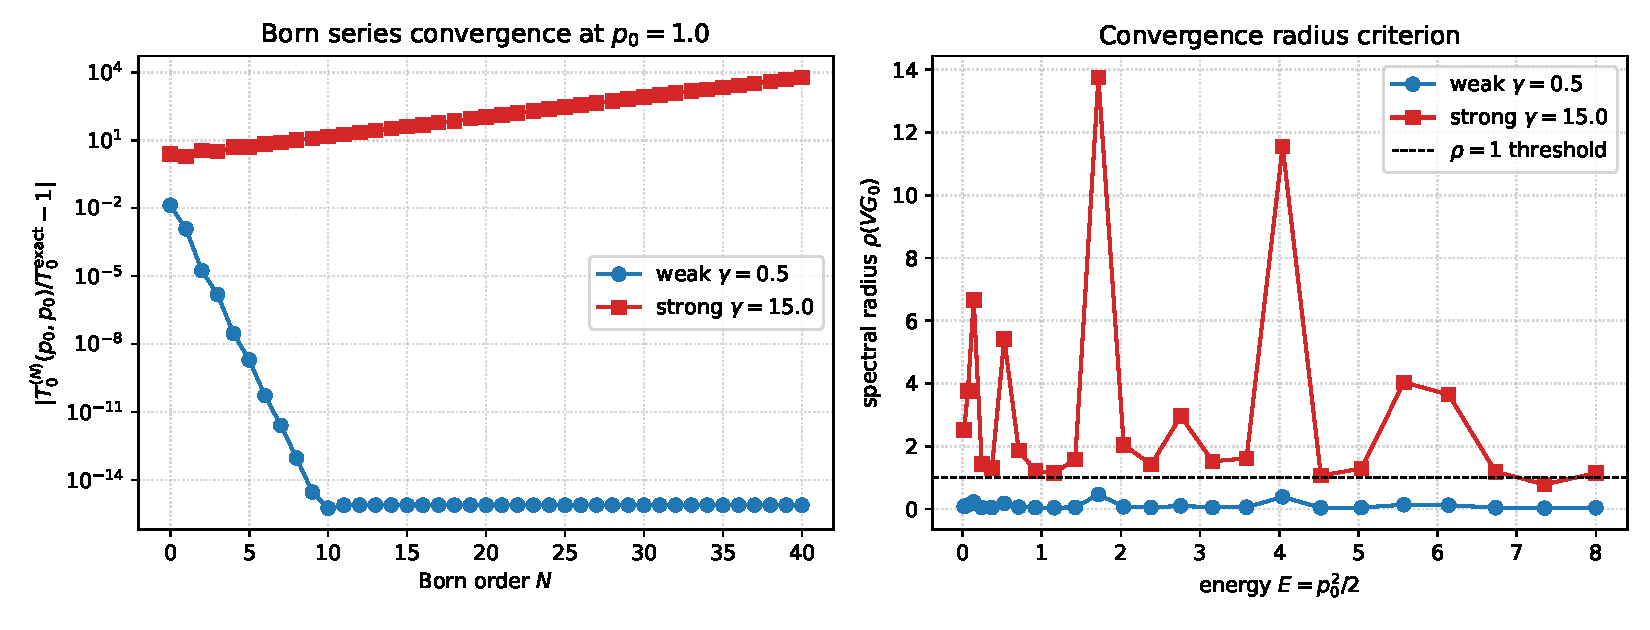
\includegraphics[width=0.95\linewidth]{ch08_born_convergence}
    \caption{Born 级数收敛性的数值验证. 左: $|T^{(N)}_{0}(p_{0},p_{0})/T_{0}^{\rm exact}-1|$
    随 Born 阶数 $N$ 的变化 (对数纵轴, $p_{0}=1$). 弱耦合 $\gamma=0.5$ (蓝色) 在 $N\sim 10$ 阶后
    达到机器精度; 强耦合 $\gamma=15$ (红色) 误差按几何方式 \emph{增大}, 表明 Born 级数发散.
    右: 算子 $VG^{0}$ 的谱半径 $\rho(VG^{0})$ 随能量 $E=p_{0}^{2}/2$ 的变化. 黑虚线为
    定理 $\rho<1$ 临界值. 弱耦合曲线一致地远在阈值之下; 强耦合曲线整体高于阈值, 且在某些能量
    出现尖峰——对应 $E$ 接近束缚态 / 共振极点时 $G^{0}$ 引起的奇异放大.}
    \label{fig:numexp-ch08}
\end{figure}

\subsection*{物理讨论}
\begin{enumerate}
\item \textbf{Born 收敛定理的数值验证.} 定理
\ref{thm:born-conv}: $\Vert VG^{0}\Vert<1$ $\Longrightarrow$ Neumann 级数
$\sum_{n}(VG^{0})^{n}$ 在算子范数下收敛. 数值实验中对应弱耦合
$\gamma=0.5$, 全能段 $\rho\sim 0.05\text{-}0.2$, 因此 $T^{(N)}\to T$ 几何收敛, 公比即谱半径——
图~\ref{fig:numexp-ch08} 左图斜率 $\log_{10}\rho\approx -0.7$ 与右图首点 $\rho_{w}\approx 0.18$
一致 (含离散化误差).
\item \textbf{束缚态阻碍全程收敛.} 强耦合 $\gamma=15$ 谱半径系统地 $>1$, 部分能量出现
$\rho\gg 1$ 的尖峰. 物理上: 当 $E$ 趋近某个束缚态能量 $E_{B}<0$ 的解析延拓投影时,
$G^{0}(p;E)$ 在被分立态 ``放大'' 的子空间贡献巨大本征值. 这与定理
\ref{thm:bound-state-block} (``束缚态阻碍 Born 级数全程收敛'') 一致, 也与本章一维 $\delta$
势例子 \eqref{eq:born-ex-delta-sum} 的几何级数公比 $\rmi mg/k$ 在 $|g|>k/m$ 时发散同源.
\item \textbf{收敛半径作为奇点指示器.} $\rho(VG^{0}(E))=1$ 的能量定义了 Born 级数的
\emph{收敛半径在能量平面上的边界}; 此边界即 $T(E)$ 作为 $E$ 的函数最近的奇点
(束缚态极点或 CDD 极点) 距离展开点的位置——这一观点正是 ch11 解析性、ch12
共振分析的出发点.
\item \textbf{重整化 / 重整求和的必要性.} 当 $\rho\geq 1$, 直接求 $T$ 必须求解线性方程
(\texttt{np.linalg.solve}) 而非作截断求和. 这正是核物理 / 多体散射中 Faddeev-AGS、
Padé 重整以及 ${\cal R}$-矩阵方法存在的根本原因: 对存在束缚 / 共振的系统, Born 级数
\emph{不是} 良定义的微扰展开.
\end{enumerate}
